\chapter{Penanganan Kesalahan}

\section{Pendahuluan}

Dalam proses pemrograman, kesalahan atau error merupakan hal yang tidak dapat dihindari. Seorang pemrogram pemula sering kali menemukan programnya berhenti tiba-tiba, menampilkan pesan kesalahan yang panjang dan membingungkan. Namun, seiring dengan meningkatnya pemahaman, kesalahan tersebut dapat dilihat bukan sebagai kegagalan, melainkan sebagai bagian penting dari proses belajar dan pengembangan perangkat lunak.

Pada dasarnya, terdapat dua jenis kesalahan utama dalam Python: \textbf{kesalahan sintaks (syntax error)} dan \textbf{kesalahan saat berjalan (runtime error)}. Kesalahan sintaks terjadi ketika penulisan kode tidak sesuai dengan aturan bahasa Python, seperti tanda kurung yang tidak seimbang atau penggunaan kata kunci yang salah—jenis kesalahan ini terdeteksi sebelum program dijalankan. Sementara itu, kesalahan saat berjalan muncul ketika program telah dieksekusi dan terjadi kondisi yang tidak diharapkan, misalnya pembagian dengan nol atau akses indeks di luar jangkauan pada sebuah \textit{list}. Kesalahan saat berjalan inilah yang, di Python, dimodelkan sebagai \textbf{exception}.

Untuk menghadapi kondisi tak terduga tersebut, Python menyediakan mekanisme \textbf{exception handling} yang memungkinkan program mengantisipasi dan menangani kesalahan tanpa harus berhenti secara mendadak. Alih-alih gagal total, program dapat menampilkan pesan yang lebih ramah, melakukan langkah pemulihan (\textit{recovery}), atau melakukan pembersihan sumber daya dengan rapi. Pada bab ini, Anda akan mempelajari cara kerja blok \texttt{try-except}, bagaimana menulis penanganan untuk \textit{banyak} jenis exception, penggunaan \texttt{else} (dijalankan ketika tidak ada error) dan \texttt{finally} (selalu dijalankan untuk \textit{cleanup}), serta cara membuat \textbf{custom exception} untuk mengekspresikan aturan domain secara lebih jelas. Tujuannya adalah agar Anda mampu menulis program Python yang \textit{robust}, informatif saat terjadi error, dan mudah dirawat.


\section{Konsep Dasar Exception}

Dalam pemrograman, kesalahan atau \textit{error} merupakan kondisi yang menyebabkan program tidak dapat berjalan sebagaimana mestinya. Python memiliki cara sistematis untuk menangani kesalahan ini agar program tetap dapat berfungsi dengan baik. Sebelum memahami bagaimana cara menanganinya, penting untuk mengetahui jenis-jenis kesalahan yang mungkin terjadi serta konsep dasar yang mendasari \textbf{exception}.

\subsection*{Kesalahan Sintaks (Syntax Error)}

Kesalahan sintaks terjadi ketika penulisan kode tidak sesuai dengan aturan bahasa Python. Interpreter Python akan mendeteksi kesalahan ini sebelum program dijalankan. Karena itu, kesalahan sintaks mencegah program untuk dieksekusi sama sekali.

\begin{lstlisting}[style=PythonStyle, caption={Contoh kesalahan sintaks}]
# Contoh kesalahan sintaks: tanda kurung kurang
print("Halo dunia"
\end{lstlisting}

Ketika dijalankan, Python akan menampilkan pesan kesalahan seperti berikut:

\begin{lstlisting}[language=bash]
SyntaxError: unexpected EOF while parsing
\end{lstlisting}

Pesan tersebut menandakan bahwa interpreter mendeteksi akhir baris yang tidak sesuai harapan — dalam hal ini, karena tanda kurung penutup tidak ada.

\subsection*{Kesalahan Saat Berjalan (Runtime Error)}

Kesalahan jenis ini hanya muncul ketika program dijalankan. Artinya, kode sudah benar secara sintaks, tetapi ketika dijalankan muncul kondisi yang tidak dapat ditangani. Contoh paling umum adalah pembagian dengan nol.

\begin{lstlisting}[style=PythonStyle, caption={Contoh kesalahan runtime}]
# Contoh kesalahan runtime: pembagian dengan nol
hasil = 10 / 0
print(hasil)
\end{lstlisting}

Ketika dijalankan, Python akan menampilkan pesan seperti berikut:

\begin{lstlisting}[language=bash]
ZeroDivisionError: division by zero
\end{lstlisting}

Berbeda dengan kesalahan sintaks, kesalahan runtime tidak menghentikan keseluruhan program secara permanen — kita dapat menangkapnya dengan mekanisme khusus agar program tetap berjalan. Kesalahan seperti inilah yang disebut \textbf{exception}.

\subsection*{Apa Itu Exception?}

\textbf{Exception} adalah peristiwa (event) yang terjadi selama eksekusi program dan mengganggu alur normal instruksi. Python memiliki berbagai jenis exception bawaan seperti:

\begin{itemize}
    \item \texttt{ZeroDivisionError} – pembagian dengan nol,
    \item \texttt{IndexError} – akses indeks list di luar jangkauan,
    \item \texttt{ValueError} – kesalahan pada nilai atau tipe data,
    \item \texttt{FileNotFoundError} – file yang diminta tidak ditemukan,
    \item \texttt{TypeError} – operasi dilakukan pada tipe data yang tidak sesuai.
\end{itemize}

Contoh berikut memperlihatkan beberapa exception umum:

\begin{lstlisting}[style=PythonStyle, caption={Beberapa contoh exception umum}]
# IndexError
angka = [1, 2, 3]
print(angka[5])

# ValueError
int("abc")

# FileNotFoundError
with open("data.txt") as f:
    isi = f.read()
\end{lstlisting}

Setiap contoh di atas akan menghasilkan jenis exception yang berbeda.

\subsection*{Mengapa Perlu Menangani Exception?}

Tanpa mekanisme penanganan exception, setiap kesalahan yang terjadi akan langsung menghentikan program. Dalam aplikasi nyata, hal ini tidak dapat diterima, terutama ketika program berinteraksi dengan pengguna atau sistem eksternal seperti file, jaringan, atau basis data. Misalnya, jika pengguna salah mengetikkan nama file, seharusnya program tidak langsung berhenti, melainkan menampilkan pesan yang ramah seperti:

\begin{lstlisting}[language=bash]
File tidak ditemukan. Silakan periksa kembali nama file Anda.
\end{lstlisting}

Penanganan exception membantu:
\begin{enumerate}
    \item Mencegah program berhenti secara tiba-tiba.
    \item Memberikan pesan kesalahan yang lebih informatif bagi pengguna.
    \item Menjaga keandalan (\textit{robustness}) dan kestabilan program.
    \item Memudahkan proses debugging dan pengujian.
\end{enumerate}

Dengan kata lain, penanganan exception adalah langkah penting menuju program yang profesional dan tangguh. Pada bagian berikutnya, kita akan mempelajari bagaimana Python menyediakan struktur \texttt{try-except} untuk menangani exception secara sistematis.


\section{Blok Try-Except}

Setelah memahami konsep dasar exception, langkah selanjutnya adalah mempelajari bagaimana Python menangani kesalahan tersebut tanpa membuat program berhenti. Untuk itu, Python menyediakan mekanisme yang disebut dengan \textbf{blok \texttt{try-except}}.

\subsection*{Struktur Dasar Try-Except}

Blok \texttt{try-except} digunakan untuk mencoba menjalankan potongan kode yang mungkin menghasilkan error, dan menangkap kesalahan tersebut jika benar terjadi. Dengan demikian, alur program tetap dapat dilanjutkan secara normal.

Struktur umumnya dapat ditulis sebagai berikut:

\begin{lstlisting}[style=PythonStyle, caption={Struktur dasar try-except di Python}]
try:
    # Kode yang mungkin menimbulkan exception
    operasi_berisiko()
except JenisException:
    # Kode yang dijalankan jika exception terjadi
    tangani_exception()
\end{lstlisting}

Alur eksekusinya sederhana:
\begin{enumerate}
    \item Python akan mengeksekusi blok \texttt{try}.
    \item Jika tidak ada kesalahan, blok \texttt{except} akan dilewati.
    \item Jika terjadi kesalahan, Python akan mencari blok \texttt{except} yang sesuai dan menjalankannya.
\end{enumerate}

Dengan cara ini, program tidak langsung berhenti saat error muncul — melainkan “menangkap” kesalahan dan bereaksi dengan cara yang lebih terkendali.

\subsection*{Contoh Sederhana Penanganan Exception}

Perhatikan contoh berikut. Kita mencoba membagi dua angka yang diinput oleh pengguna, tetapi bisa saja pengguna memasukkan nilai nol yang menyebabkan error pembagian.

\begin{lstlisting}[style=PythonStyle, caption={Contoh sederhana penggunaan try-except}]
try:
    a = int(input("Masukkan angka pertama: "))
    b = int(input("Masukkan angka kedua: "))
    hasil = a / b
    print("Hasil pembagian:", hasil)
except ZeroDivisionError:
    print("Error: Tidak dapat membagi dengan nol!")
\end{lstlisting}

Jika pengguna memasukkan nilai kedua sebagai nol, maka keluaran program akan seperti berikut:

\begin{lstlisting}[language=bash]
Masukkan angka pertama: 10
Masukkan angka kedua: 0
Error: Tidak dapat membagi dengan nol!
\end{lstlisting}

Sedangkan jika pengguna memasukkan dua angka valid, program akan menampilkan hasil pembagiannya tanpa gangguan.

\begin{lstlisting}[language=bash]
Masukkan angka pertama: 10
Masukkan angka kedua: 2
Hasil pembagian: 5.0
\end{lstlisting}

Dengan demikian, meskipun terjadi kesalahan, program tidak berhenti secara tiba-tiba — melainkan menampilkan pesan kesalahan yang lebih mudah dipahami pengguna.

\subsection*{Menangkap Semua Jenis Kesalahan}

Kadang kita tidak tahu secara pasti jenis kesalahan apa yang akan terjadi. Dalam kasus seperti itu, kita dapat menangkap semua jenis exception tanpa menyebutkan nama exception-nya.

\begin{lstlisting}[style=PythonStyle, caption={Menangkap semua jenis exception}]
try:
    x = int(input("Masukkan angka: "))
    y = 10 / x
    print("Hasil:", y)
except:
    print("Terjadi kesalahan yang tidak diketahui.")
\end{lstlisting}

Namun, praktik ini \textbf{tidak disarankan} untuk program besar, karena menyulitkan proses debugging — kita tidak tahu jenis kesalahan apa yang sebenarnya terjadi. Sebaiknya selalu tangani exception yang spesifik bila memungkinkan.

\subsection*{Menggunakan Pesan Error Kustom}

Selain menampilkan pesan umum, kita dapat menampilkan pesan yang lebih informatif dengan menangkap objek exception. Python memungkinkan kita mendapatkan detail error melalui kata kunci \texttt{as}.

\begin{lstlisting}[style=PythonStyle, caption={Penggunaan pesan error kustom}]
try:
    nama_file = input("Masukkan nama file: ")
    with open(nama_file) as f:
        isi = f.read()
        print("Isi file:", isi)
except FileNotFoundError as e:
    print("Terjadi kesalahan:", e)
    print("File tidak ditemukan. Silakan periksa nama file Anda.")
\end{lstlisting}

Contoh hasil eksekusi ketika pengguna memasukkan nama file yang salah:

\begin{lstlisting}[language=bash]
Masukkan nama file: data_tidak_ada.txt
Terjadi kesalahan: [Errno 2] No such file or directory: 'data_tidak_ada.txt'
File tidak ditemukan. Silakan periksa nama file Anda.
\end{lstlisting}

Dengan menampilkan pesan bawaan dari Python sekaligus menambahkan penjelasan sendiri, kita dapat membantu pengguna memahami sumber masalah sekaligus memberi arahan yang jelas.

\subsection*{Kesimpulan}

Blok \texttt{try-except} merupakan pondasi utama dalam penanganan kesalahan di Python. Ia memungkinkan program untuk:
\begin{itemize}
    \item Tetap berjalan meskipun terjadi error,
    \item Menyediakan pesan kesalahan yang ramah dan informatif,
    \item Mengontrol perilaku program saat situasi tak terduga muncul.
\end{itemize}

Pada bagian selanjutnya, kita akan memperluas konsep ini dengan menangani \textbf{beberapa jenis exception sekaligus} serta mempelajari bagaimana menambahkan blok tambahan seperti \texttt{else} dan \texttt{finally} untuk pengendalian alur yang lebih fleksibel.


\section{Menangani Beberapa Jenis Exception}

Dalam praktiknya, satu potongan kode bisa saja berpotensi menimbulkan berbagai jenis kesalahan. Misalnya, kesalahan input pengguna, pembagian dengan nol, atau file yang tidak ditemukan. Untuk menghadapi kondisi tersebut, Python memungkinkan kita menulis beberapa blok \texttt{except} agar setiap jenis exception dapat ditangani secara berbeda sesuai konteksnya.

\subsection*{Menangani Beberapa Exception Secara Terpisah}

Kita dapat menambahkan lebih dari satu blok \texttt{except} untuk menangani jenis kesalahan yang berbeda-beda. Dengan cara ini, program dapat memberikan respon yang lebih tepat sesuai dengan situasi yang terjadi.

\begin{lstlisting}[style=PythonStyle, caption={Menangani beberapa exception secara terpisah}]
try:
    a = int(input("Masukkan angka pertama: "))
    b = int(input("Masukkan angka kedua: "))
    hasil = a / b
    print("Hasil pembagian:", hasil)
except ZeroDivisionError:
    print("Error: Tidak dapat membagi dengan nol.")
except ValueError:
    print("Error: Input harus berupa angka, bukan teks.")
\end{lstlisting}

Berikut contoh hasil eksekusinya:

\begin{lstlisting}[language=bash]
Masukkan angka pertama: 10
Masukkan angka kedua: 0
Error: Tidak dapat membagi dengan nol.
\end{lstlisting}

\begin{lstlisting}[language=bash]
Masukkan angka pertama: sepuluh
Masukkan angka kedua: 2
Error: Input harus berupa angka, bukan teks.
\end{lstlisting}

Dengan pendekatan ini, setiap error yang berbeda dapat ditangani dengan cara yang lebih spesifik, sehingga pengguna mendapatkan informasi yang lebih akurat.

\subsection*{Menggabungkan Beberapa Exception dalam Satu Blok}

Terkadang beberapa jenis exception dapat ditangani dengan cara yang sama. Untuk kasus seperti ini, Python memungkinkan kita menulis beberapa nama exception dalam satu blok \texttt{except} menggunakan tanda kurung.

\begin{lstlisting}[style=PythonStyle, caption={Menggabungkan beberapa exception dalam satu blok}]
try:
    nilai = int(input("Masukkan angka: "))
    hasil = 100 / nilai
    print("Hasil:", hasil)
except (ZeroDivisionError, ValueError):
    print("Error: Input tidak valid atau pembagian dengan nol.")
\end{lstlisting}

Hasilnya akan sama baik ketika pengguna memasukkan nilai nol maupun teks yang tidak bisa diubah menjadi angka:

\begin{lstlisting}[language=bash]
Masukkan angka: 0
Error: Input tidak valid atau pembagian dengan nol.
\end{lstlisting}

\begin{lstlisting}[language=bash]
Masukkan angka: abc
Error: Input tidak valid atau pembagian dengan nol.
\end{lstlisting}

Teknik ini berguna ketika penanganan kedua jenis kesalahan cukup serupa dan tidak perlu dibedakan secara eksplisit.

\subsection*{Hierarki Exception di Python}

Python memiliki sistem hierarki exception di mana semua jenis kesalahan diturunkan dari kelas dasar \texttt{BaseException}. Sebagian besar exception yang sering kita tangani berasal dari turunan \texttt{Exception}.  
Gambaran sederhananya sebagai berikut:

\begin{center}
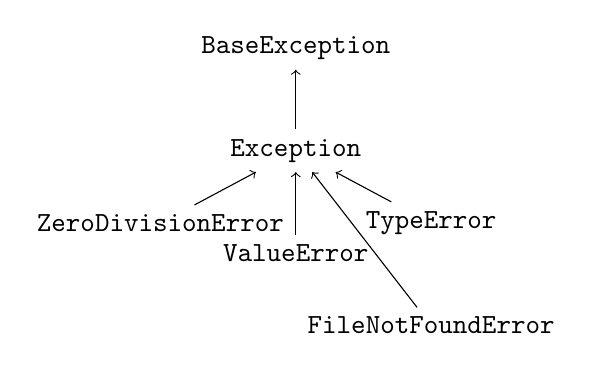
\begin{tikzpicture}[node distance=1.3cm, every node/.style={font=\ttfamily}]
\node (base) {BaseException};
\node (exc) [below of=base] {Exception};
\node (zero) [below left of=exc, xshift=-0.8cm] {ZeroDivisionError};
\node (value) [below of=exc] {ValueError};
\node (type) [below right of=exc, xshift=0.8cm] {TypeError};
\node (file) [below right of=value, xshift=0.8cm] {FileNotFoundError};
\draw[->] (exc) -- (base);
\draw[->] (zero) -- (exc);
\draw[->] (value) -- (exc);
\draw[->] (type) -- (exc);
\draw[->] (file) -- (exc);
\end{tikzpicture}
\end{center}

Artinya, jika kita menangkap \texttt{Exception} saja, maka semua jenis kesalahan yang merupakan turunannya juga akan tertangkap. Namun, untuk alasan kejelasan dan debugging yang efektif, sebaiknya kita menangkap jenis exception yang spesifik.

\begin{lstlisting}[style=PythonStyle, caption={Menangkap seluruh exception menggunakan kelas induk}]
try:
    x = int("abc")  # menyebabkan ValueError
except Exception as e:
    print("Terjadi kesalahan:", e)
\end{lstlisting}

Keluaran program:

\begin{lstlisting}[language=bash]
Terjadi kesalahan: invalid literal for int() with base 10: 'abc'
\end{lstlisting}

Dengan menangkap kelas induk \texttt{Exception}, semua jenis kesalahan turunan akan tertangani, tetapi kita tetap dapat mengakses detail error melalui variabel \texttt{e}.

\subsection*{Menggunakan \texttt{as} untuk Mendapatkan Objek Exception}

Dalam contoh sebelumnya, kita telah melihat bahwa kata kunci \texttt{as} digunakan untuk menangkap objek exception dan menyimpannya dalam variabel. Objek ini berisi informasi penting seperti pesan error, nama exception, dan atribut tambahan lainnya.

\begin{lstlisting}[style=PythonStyle, caption={Menggunakan 'as' untuk menangkap objek exception}]
try:
    angka = int(input("Masukkan angka: "))
    hasil = 100 / angka
    print("Hasil:", hasil)
except Exception as e:
    print("Tipe kesalahan:", type(e).__name__)
    print("Pesan kesalahan:", e)
\end{lstlisting}

Contoh hasil ketika pengguna memasukkan nilai nol:

\begin{lstlisting}[language=bash]
Masukkan angka: 0
Tipe kesalahan: ZeroDivisionError
Pesan kesalahan: division by zero
\end{lstlisting}

Atau jika pengguna memasukkan teks:

\begin{lstlisting}[language=bash]
Masukkan angka: abc
Tipe kesalahan: ValueError
Pesan kesalahan: invalid literal for int() with base 10: 'abc'
\end{lstlisting}

Dengan teknik ini, kita dapat menampilkan pesan yang lebih dinamis, mencatat error ke log, atau mengambil keputusan program secara otomatis berdasarkan jenis kesalahan yang terjadi.

\subsection*{Kesimpulan}

Pada bagian ini, kita telah mempelajari cara menangani lebih dari satu jenis exception, memahami hierarki exception di Python, dan menggunakan objek exception untuk memperoleh informasi lebih lanjut.  
Pendekatan ini membuat kode lebih \textit{robust}, mudah dirawat, serta lebih ramah bagi pengguna.  

Selanjutnya, kita akan membahas dua blok tambahan dalam penanganan exception, yaitu \texttt{else} dan \texttt{finally}, yang memberikan fleksibilitas lebih dalam mengontrol alur program.


\section{Blok Else dan Finally}

Selain blok \texttt{try} dan \texttt{except}, Python juga menyediakan dua blok tambahan yang dapat digunakan untuk mengontrol alur program secara lebih fleksibel, yaitu \texttt{else} dan \texttt{finally}. Kedua blok ini tidak wajib digunakan, tetapi sangat berguna untuk situasi tertentu, terutama ketika kita ingin memisahkan logika normal dari logika penanganan kesalahan, atau ketika kita perlu memastikan bahwa suatu tindakan pembersihan (\textit{cleanup}) tetap dilakukan meskipun terjadi error.

\subsection*{Blok Else}

Blok \texttt{else} digunakan setelah \texttt{except}, dan hanya akan dijalankan jika tidak terjadi exception dalam blok \texttt{try}. Dengan kata lain, kode di dalam \texttt{else} hanya berjalan ketika semua operasi di \texttt{try} berhasil.

Struktur lengkapnya sebagai berikut:

\begin{lstlisting}[style=PythonStyle, caption={Struktur lengkap try-except-else}]
try:
    # kode utama yang mungkin menyebabkan exception
except JenisException:
    # penanganan error
else:
    # kode ini hanya berjalan jika tidak ada error
\end{lstlisting}

Contoh penerapan:

\begin{lstlisting}[style=PythonStyle, caption={Penggunaan blok else}]
try:
    angka = int(input("Masukkan angka: "))
    hasil = 100 / angka
except ZeroDivisionError:
    print("Error: Pembagian dengan nol tidak diperbolehkan.")
except ValueError:
    print("Error: Input harus berupa angka.")
else:
    print("Hasil perhitungan:", hasil)
\end{lstlisting}

Hasil eksekusi ketika pengguna memasukkan angka valid:

\begin{lstlisting}[language=bash]
Masukkan angka: 5
Hasil perhitungan: 20.0
\end{lstlisting}

Dan ketika terjadi error:

\begin{lstlisting}[language=bash]
Masukkan angka: 0
Error: Pembagian dengan nol tidak diperbolehkan.
\end{lstlisting}

Blok \texttt{else} sangat bermanfaat untuk memisahkan logika utama dari logika penanganan error. Dengan begitu, struktur kode menjadi lebih bersih dan mudah dibaca.

\subsection*{Blok Finally}

Blok \texttt{finally} berfungsi untuk mengeksekusi kode yang harus dijalankan dalam kondisi apa pun — baik terjadi error maupun tidak. Biasanya, blok ini digunakan untuk melakukan tindakan pembersihan (\textit{cleanup}) seperti menutup file, melepaskan koneksi jaringan, atau menghapus data sementara.

\begin{lstlisting}[style=PythonStyle, caption={Struktur penggunaan blok finally}]
try:
    # operasi utama
except:
    # penanganan kesalahan
finally:
    # selalu dijalankan, baik ada error maupun tidak
\end{lstlisting}

Contoh penerapan nyata: membaca file dan memastikan file selalu ditutup.

\begin{lstlisting}[style=PythonStyle, caption={Contoh penggunaan finally untuk pembersihan}]
try:
    f = open("data.txt", "r")
    isi = f.read()
    print("Isi file:", isi)
except FileNotFoundError:
    print("Error: File tidak ditemukan.")
finally:
    print("Menutup file...")
    f.close()
\end{lstlisting}

Jika file tidak ditemukan, maka hasilnya:

\begin{lstlisting}[language=bash]
Error: File tidak ditemukan.
Menutup file...
Traceback (most recent call last):
  File "contoh.py", line 8, in <module>
    f.close()
UnboundLocalError: local variable 'f' referenced before assignment
\end{lstlisting}

Terjadi error baru karena variabel \texttt{f} belum pernah dibuat. Untuk menghindarinya, sebaiknya kita melakukan pemeriksaan terlebih dahulu sebelum menutup file.

\begin{lstlisting}[style=PythonStyle, caption={Menangani variabel dengan aman di finally}]
f = None
try:
    f = open("data.txt", "r")
    isi = f.read()
    print("Isi file:", isi)
except FileNotFoundError:
    print("Error: File tidak ditemukan.")
finally:
    if f is not None:
        f.close()
        print("File berhasil ditutup.")
\end{lstlisting}

Hasil keluaran saat file tidak ada:

\begin{lstlisting}[language=bash]
Error: File tidak ditemukan.
\end{lstlisting}

Dan ketika file ada:

\begin{lstlisting}[language=bash]
Isi file: Halo, ini contoh isi file.
File berhasil ditutup.
\end{lstlisting}

Dengan menggunakan \texttt{finally}, kita menjamin bahwa tindakan penting seperti menutup file selalu dilakukan, terlepas dari apakah program mengalami kesalahan atau tidak.

\subsection*{Diagram Alur Try-Except-Else-Finally}

Berikut diagram sederhana untuk menggambarkan alur eksekusi blok-blok tersebut:

\begin{center}
\begin{tikzpicture}[node distance=1.5cm, font=\small, align=center]
\node (start) [draw, rounded corners] {\textbf{Mulai}};
\node (try) [below of=start, draw, rounded corners, fill=blue!5] {\textbf{Blok try}};
\node (error?) [below of=try, draw, diamond, aspect=2, fill=yellow!10] {\textbf{Terjadi Exception?}};
\node (except) [below left of=error?, xshift=-1.2cm, draw, rounded corners, fill=red!10] {\textbf{Blok except}};
\node (else) [below right of=error?, xshift=1.2cm, draw, rounded corners, fill=green!10] {\textbf{Blok else}};
\node (finally) [below of=error?, yshift=-.5cm, draw, rounded corners, fill=orange!10] {\textbf{Blok finally}};
\node (end) [below of=finally, draw, rounded corners] {\textbf{Selesai}};

\draw[->] (start) -- (try);
\draw[->] (try) -- (error?);
\draw[->] (error?) -- node[left]{\textbf{Ya}} (except);
\draw[->] (error?) -- node[right]{\textbf{Tidak}} (else);
\draw[->] (except) |- (finally);
\draw[->] (else) |- (finally);
\draw[->] (finally) -- (end);
\end{tikzpicture}
\end{center}

Diagram di atas menunjukkan bahwa blok \texttt{finally} selalu dijalankan, baik ada exception maupun tidak.

\subsection*{Kesimpulan}

Blok \texttt{else} dan \texttt{finally} membantu kita menulis kode Python yang lebih rapi, aman, dan terstruktur:
\begin{itemize}
    \item Gunakan \texttt{else} untuk kode yang hanya perlu dijalankan jika tidak ada error.
    \item Gunakan \texttt{finally} untuk tindakan pembersihan yang wajib dilakukan.
\end{itemize}

Kombinasi empat blok ini — \texttt{try}, \texttt{except}, \texttt{else}, dan \texttt{finally} — memberi kendali penuh terhadap perilaku program dalam menghadapi kesalahan dan proses penyelesaian.


\section{Membuat Exception Sendiri}

Selain menggunakan berbagai jenis exception bawaan Python seperti \texttt{ValueError} atau \texttt{ZeroDivisionError}, kita juga dapat membuat jenis exception kita sendiri yang sesuai dengan kebutuhan program. Kemampuan ini berguna ketika kita ingin mendefinisikan kesalahan yang bersifat lebih spesifik dan bermakna sesuai konteks aplikasi yang kita kembangkan.

\subsection*{Pengenalan Custom Exception}

\textbf{Custom exception} atau pengecualian buatan sendiri memungkinkan kita membuat tipe kesalahan baru dengan pesan dan perilaku yang kita tentukan. Biasanya, custom exception digunakan untuk situasi yang tidak tercakup oleh exception standar Python.

Sebagai contoh, dalam sebuah aplikasi keuangan, kita mungkin ingin membuat kesalahan khusus seperti \texttt{SaldoTidakCukupError} atau \texttt{TransaksiTidakValidError}. Hal ini membuat kode lebih mudah dibaca dan dipahami, karena jenis error langsung menggambarkan konteks masalahnya.

\subsection*{Cara Mendefinisikan Class Exception Sendiri}

Untuk membuat exception baru, kita cukup mendefinisikan kelas Python yang diturunkan (\textit{inherit}) dari kelas dasar \texttt{Exception}. Kita juga dapat menambahkan konstruktor khusus atau atribut tambahan sesuai kebutuhan.

\begin{lstlisting}[style=PythonStyle, caption={Contoh mendefinisikan custom exception sederhana}]
class InputNegatifError(Exception):
    """Exception yang muncul jika input bernilai negatif."""
    pass

# Contoh penggunaan
def hitung_akar(x):
    if x < 0:
        raise InputNegatifError("Tidak bisa menghitung akar dari bilangan negatif!")
    return x ** 0.5

try:
    angka = int(input("Masukkan angka: "))
    print("Hasil akar:", hitung_akar(angka))
except InputNegatifError as e:
    print("Terjadi kesalahan:", e)
\end{lstlisting}

Ketika pengguna memasukkan angka negatif, hasilnya akan seperti berikut:

\begin{lstlisting}[language=bash]
Masukkan angka: -9
Terjadi kesalahan: Tidak bisa menghitung akar dari bilangan negatif!
\end{lstlisting}

Dalam contoh ini, kita menggunakan \texttt{raise} untuk “melempar” exception buatan sendiri ketika kondisi tidak valid terdeteksi.  
Mekanisme ini sangat berguna untuk mengendalikan alur logika program secara terstruktur.

\subsection*{Menambahkan Atribut dan Konstruktor Khusus}

Kita juga dapat menambahkan informasi tambahan pada exception buatan sendiri, misalnya nilai input yang menyebabkan error, atau pesan khusus yang dapat diproses lebih lanjut.

\begin{lstlisting}[style=PythonStyle, caption={Custom exception dengan atribut tambahan}]
class NilaiTidakValidError(Exception):
    """Exception untuk nilai yang berada di luar rentang tertentu."""
    def __init__(self, nilai, pesan="Nilai di luar rentang yang diperbolehkan."):
        self.nilai = nilai
        self.pesan = pesan
        super().__init__(self.pesan)

def set_nilai(nilai):
    if nilai < 0 or nilai > 100:
        raise NilaiTidakValidError(nilai)
    print(f"Nilai {nilai} disimpan dengan sukses.")

try:
    set_nilai(150)
except NilaiTidakValidError as e:
    print(f"Error: {e.pesan} (nilai: {e.nilai})")
\end{lstlisting}

Keluaran program:

\begin{lstlisting}[language=bash]
Error: Nilai di luar rentang yang diperbolehkan. (nilai: 150)
\end{lstlisting}

Dengan menambahkan atribut seperti \texttt{nilai}, kita dapat melacak konteks kesalahan dengan lebih detail.

\subsection*{Studi Kasus: Validasi Input Pengguna}

Sebagai ilustrasi penerapan nyata, perhatikan contoh berikut: kita akan membuat sistem sederhana yang meminta pengguna memasukkan usia. Program harus menolak nilai yang tidak masuk akal, seperti angka negatif atau usia lebih dari 120 tahun, dengan menggunakan custom exception.

\begin{lstlisting}[style=PythonStyle, caption={Studi kasus: validasi input usia dengan custom exception}]
class UsiaTidakValidError(Exception):
    """Exception untuk usia yang tidak logis."""
    def __init__(self, usia, pesan="Usia tidak valid."):
        self.usia = usia
        self.pesan = pesan
        super().__init__(self.pesan)

def input_usia():
    usia = int(input("Masukkan usia Anda: "))
    if usia < 0:
        raise UsiaTidakValidError(usia, "Usia tidak boleh negatif.")
    elif usia > 120:
        raise UsiaTidakValidError(usia, "Usia terlalu besar untuk manusia.")
    return usia

try:
    umur = input_usia()
    print("Usia Anda adalah:", umur)
except UsiaTidakValidError as e:
    print(f"Error: {e.pesan} (diberikan: {e.usia})")
except ValueError:
    print("Error: Input harus berupa angka.")
\end{lstlisting}

Keluaran contoh:

\begin{lstlisting}[language=bash]
Masukkan usia Anda: -5
Error: Usia tidak boleh negatif. (diberikan: -5)
\end{lstlisting}

Atau:

\begin{lstlisting}[language=bash]
Masukkan usia Anda: 130
Error: Usia terlalu besar untuk manusia. (diberikan: 130)
\end{lstlisting}

Dan jika pengguna memasukkan nilai yang valid:

\begin{lstlisting}[language=bash]
Masukkan usia Anda: 25
Usia Anda adalah: 25
\end{lstlisting}

\subsection*{Manfaat Membuat Exception Sendiri}

Dengan menggunakan custom exception, kita mendapatkan beberapa keuntungan penting:
\begin{itemize}
    \item Kode lebih mudah dibaca karena jenis error menggambarkan konteks spesifik masalah.
    \item Memisahkan kesalahan logika bisnis dari error teknis bawaan Python.
    \item Memudahkan proses debugging dan pelaporan error.
    \item Meningkatkan fleksibilitas dalam menangani kondisi yang tidak biasa.
\end{itemize}

\subsection*{Kesimpulan}

Custom exception memberi kemampuan bagi pengembang untuk mendefinisikan kesalahan sesuai kebutuhan domain aplikasinya.  
Dengan mendefinisikan kelas exception sendiri, kita dapat membuat program yang lebih \textit{robust}, mudah dipelihara, dan kaya informasi saat terjadi kesalahan.

Pada bagian berikutnya, kita akan memperluas topik ini dengan membahas konsep penting berikutnya dalam pengembangan perangkat lunak yang andal — yaitu \textbf{pengujian unit (unit testing)} menggunakan modul \texttt{unittest}.



\section{Latihan}

Bagian ini bertujuan untuk membantu Anda berlatih memahami dan menerapkan konsep \textbf{penanganan kesalahan (exception handling)} dalam Python.  
Setiap soal dirancang untuk memperkuat pemahaman Anda terhadap berbagai aspek seperti penggunaan \texttt{try-except}, \texttt{else}, \texttt{finally}, serta pembuatan \textit{custom exception}.

\subsection*{Latihan Dasar}

\begin{enumerate}
    \item \textbf{Menangani Pembagian Nol}  
    Buatlah sebuah program yang meminta dua input angka dari pengguna dan menampilkan hasil pembagian dari keduanya.  
    Gunakan blok \texttt{try-except} untuk menangani kesalahan \texttt{ZeroDivisionError}.  
    Jika pengguna memasukkan nol sebagai penyebut, tampilkan pesan:  
    \texttt{"Error: Pembagian dengan nol tidak diperbolehkan."}

    \item \textbf{Validasi Input Angka}  
    Tulis program yang meminta pengguna memasukkan sebuah angka bulat.  
    Jika input bukan angka, tangkap kesalahan \texttt{ValueError} dan tampilkan pesan kesalahan yang ramah.  
    Gunakan \texttt{else} untuk mencetak nilai yang berhasil dimasukkan.

    \item \textbf{Membaca File dengan Aman}  
    Buat program yang mencoba membaca isi file berdasarkan nama yang dimasukkan pengguna.  
    Tangani kemungkinan kesalahan \texttt{FileNotFoundError}, dan gunakan \texttt{finally} untuk menampilkan pesan:  
    \texttt{"Operasi selesai, terima kasih."}
\end{enumerate}

\subsection*{Latihan Menengah}

\begin{enumerate}
    \item \textbf{Menangani Beberapa Jenis Exception}  
    Buat program yang meminta pengguna memasukkan dua angka, lalu melakukan operasi pembagian.  
    Tangani dua kemungkinan error:
    \begin{itemize}
        \item \texttt{ValueError} – jika pengguna tidak memasukkan angka.
        \item \texttt{ZeroDivisionError} – jika penyebut bernilai nol.
    \end{itemize}
    Tambahkan blok \texttt{else} untuk mencetak hasil jika tidak ada kesalahan, dan blok \texttt{finally} untuk menampilkan pesan “Selesai memproses data.”

    \item \textbf{Membuat Custom Exception}  
    Buat kelas exception baru bernama \texttt{NilaiNegatifError} yang muncul jika input pengguna berupa angka negatif.  
    Gunakan exception ini dalam fungsi \texttt{cek\_positif(n)} yang akan menolak angka negatif dengan pesan error:  
    \texttt{"Nilai tidak boleh negatif!"}  
    Tampilkan contoh penggunaan fungsi ini dalam blok \texttt{try-except}.
\end{enumerate}

\subsection*{Tantangan Lanjutan}

\begin{enumerate}
    \item \textbf{Validasi Formulir Sederhana}  
    Buat program yang mensimulasikan pengisian formulir dengan tiga input:
    \begin{itemize}
        \item Nama (tidak boleh kosong),
        \item Usia (harus antara 0–120),
        \item Email (harus mengandung karakter '@').
    \end{itemize}
    Buat tiga \textit{custom exception}:
    \begin{itemize}
        \item \texttt{NamaKosongError},
        \item \texttt{UsiaTidakValidError},
        \item \texttt{EmailTidakValidError}.
    \end{itemize}
    Gunakan ketiga exception tersebut untuk memvalidasi data pengguna dan tampilkan pesan kesalahan yang sesuai jika ada input yang tidak valid.

    \item \textbf{Simulasi ATM Sederhana}  
    Buat program simulasi ATM dengan fitur:
    \begin{itemize}
        \item Pengguna dapat memasukkan saldo awal.
        \item Pengguna dapat melakukan penarikan sejumlah uang.
    \end{itemize}
    Buat exception baru bernama \texttt{SaldoTidakCukupError} yang muncul jika pengguna mencoba menarik saldo lebih besar dari jumlah yang tersedia.  
    Gunakan blok \texttt{try-except-finally} untuk menampilkan pesan saldo akhir meskipun terjadi kesalahan.

    \item \textbf{Menangkap dan Menulis Log Kesalahan}  
    Buat program yang menjalankan beberapa operasi aritmetika dari daftar, seperti pembagian, akar kuadrat, dan konversi tipe data.  
    Jika terjadi exception, tangkap semua jenis kesalahan (\texttt{Exception}) dan tulis pesan error ke file bernama \texttt{error.log}.  
    Setiap baris log harus memuat waktu kejadian dan jenis error yang terjadi.
\end{enumerate}

\subsection*{Refleksi}

Setelah menyelesaikan latihan di atas, renungkan pertanyaan berikut:
\begin{itemize}
    \item Mengapa penting untuk menangani kesalahan secara eksplisit?
    \item Dalam situasi apa sebaiknya kita menggunakan custom exception?
    \item Bagaimana penanganan exception dapat meningkatkan pengalaman pengguna (\textit{user experience})?
\end{itemize}

Latihan-latihan ini diharapkan dapat membantu Anda memahami konsep dasar hingga lanjutan dari penanganan kesalahan, serta menyiapkan landasan kuat sebelum mempelajari topik selanjutnya: \textbf{pengujian unit (unit testing)}.


\section{Ringkasan}

Pada bab ini, Anda telah mempelajari bahwa kesalahan (\textit{error}) adalah bagian alami dari pemrograman dan dapat ditangani secara elegan menggunakan mekanisme \textbf{exception}. Kita membedakan antara \textit{syntax error} (terdeteksi sebelum eksekusi) dan \textit{runtime error}/\textbf{exception} (muncul saat program berjalan). Dengan blok \texttt{try-except}, alur program tidak perlu terhenti; Anda dapat memberikan pesan yang ramah, mengambil tindakan pemulihan, dan menjaga pengalaman pengguna. Kita juga meninjau pola lanjut seperti \texttt{else} (dijalankan saat tidak ada error) dan \texttt{finally} (selalu dijalankan untuk \textit{cleanup}), serta menangani banyak jenis exception secara spesifik agar debugging lebih mudah dan kode lebih jelas. Selain itu, Anda belajar membuat \textbf{custom exception} untuk mengekspresikan aturan bisnis/domain secara eksplisit.

Fondasi ini menjadi pasangan erat bagi praktik \textbf{pengujian} dalam pengembangan perangkat lunak yang andal. Dengan pemahaman exception handling yang kuat, Anda siap melangkah ke pengujian otomatis (misalnya dengan \texttt{unittest}) guna memverifikasi perilaku fungsi, mencegah regresi, dan mempertahankan kualitas kode seiring perubahan. Intinya: gunakan \texttt{try-except-else-finally} untuk mengendalikan alur saat terjadi kondisi tak terduga, manfaatkan exception yang spesifik (atau custom) untuk kejelasan, dan lengkapi dengan pengujian yang baik agar program tetap \textit{robust}, mudah dirawat, dan dapat diandalkan.
